\documentclass[crop,tikz]{standalone}
\usetikzlibrary{arrows.meta}

\begin{document}
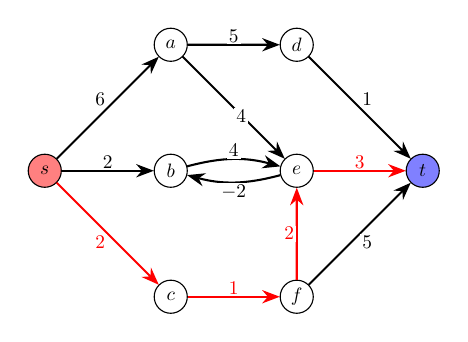
\begin{tikzpicture}[scale=.8,every node/.style={scale=.7},font=\ttfamily,
  vertex/.style={circle,draw,minimum size=6mm,inner sep=0},
  edge/.style={-Stealth,line width=.75pt},
  lab/.style={fill=white,inner sep=1pt}]
  \foreach \name/\x/\y/\fill in {
    s/0/0/red!50,a/2/2/white,b/2/0/white,c/2/-2/white,
    d/4/2/white,e/4/0/white,f/4/-2/white,t/6/0/blue!50}
    \node[vertex,fill=\fill] (\name) at (\x,\y) {$\name$};

  \foreach \a/\b/\w/\pos in {
    s/a/6/above left,s/b/2/above,a/d/5/above,a/e/4/below right,
    d/t/1/above right,f/t/5/below right} {
    \draw[edge] (\a) -- node[lab,\pos] {$\w$} (\b);
  }
  \foreach \a/\b/\w/\pos in {s/c/2/below left,c/f/1/above,e/t/3/above,f/e/2/left} {
    \draw[edge,red] (\a) -- node[lab,\pos,text=red] {$\w$} (\b);
  }
  \draw[edge,bend left=15] (b) to node[lab,above] {$4$} (e);
  \draw[edge,bend left=15] (e) to node[lab,below] {$-2$} (b);
\end{tikzpicture}
\end{document}
